\documentclass[tikz,border=10pt]{standalone}
\usetikzlibrary{calc}
\usetikzlibrary{decorations.pathmorphing}
\usetikzlibrary{intersections}
\makeatletter

% gluon decoration (based on the original coil decoration)
\pgfdeclaredecoration{gluon}{coil}
{
  \state{coil}[switch if less than=%
    0.5\pgfdecorationsegmentlength+%>
    \pgfdecorationsegmentaspect\pgfdecorationsegmentamplitude+%
    \pgfdecorationsegmentaspect\pgfdecorationsegmentamplitude to last,
               width=+\pgfdecorationsegmentlength]
  {
    \pgfpathcurveto
    {\pgfpoint@oncoil{0    }{ 0.555}{1}}
    {\pgfpoint@oncoil{0.445}{ 1    }{2}}
    {\pgfpoint@oncoil{1    }{ 1    }{3}}
    \pgfpathcurveto
    {\pgfpoint@oncoil{1.555}{ 1    }{4}}
    {\pgfpoint@oncoil{2    }{ 0.555}{5}}
    {\pgfpoint@oncoil{2    }{ 0    }{6}}
    \pgfpathcurveto
    {\pgfpoint@oncoil{2    }{-0.555}{7}}
    {\pgfpoint@oncoil{1.555}{-1    }{8}}
    {\pgfpoint@oncoil{1    }{-1    }{9}}
    \pgfpathcurveto
    {\pgfpoint@oncoil{0.445}{-1    }{10}}
    {\pgfpoint@oncoil{0    }{-0.555}{11}}
    {\pgfpoint@oncoil{0    }{ 0    }{12}}
  }
  \state{last}[next state=final]
  {
    \pgfpathcurveto
    {\pgfpoint@oncoil{0    }{ 0.555}{1}}
    {\pgfpoint@oncoil{0.445}{ 1    }{2}}
    {\pgfpoint@oncoil{1    }{ 1    }{3}}
    \pgfpathcurveto
    {\pgfpoint@oncoil{1.555}{ 1    }{4}}
    {\pgfpoint@oncoil{2    }{ 0.555}{5}}
    {\pgfpoint@oncoil{2    }{ 0    }{6}}
  }
  \state{final}{}
}

\def\pgfpoint@oncoil#1#2#3{%
  \pgf@x=#1\pgfdecorationsegmentamplitude%
  \pgf@x=\pgfdecorationsegmentaspect\pgf@x%
  \pgf@y=#2\pgfdecorationsegmentamplitude%
  \pgf@xa=0.083333333333\pgfdecorationsegmentlength%
  \advance\pgf@x by#3\pgf@xa%
}

\makeatother


\begin{document}
  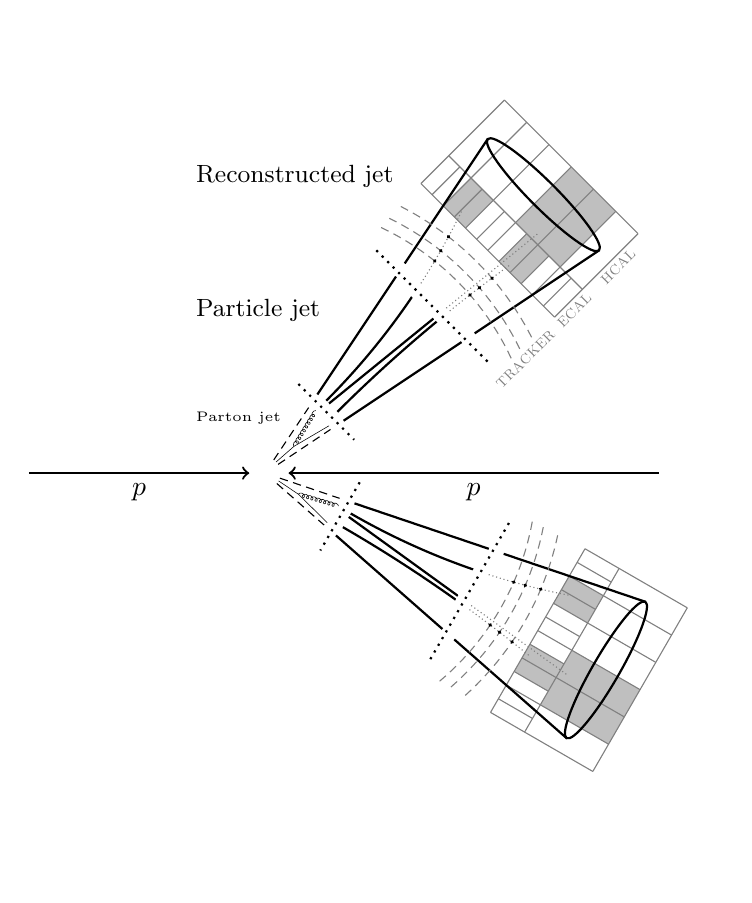
\begin{tikzpicture}
    % \draw [<->,thick] (-6,0) -- (6,0) node (yaxis) [above] {$z$};
    % \draw [<->,thick] (0,-4) -- (0,4) node (yaxis) [above] {$y$};
    \draw[thick, ->] (-3,0) -- (-0.2,0) node[below, midway] {$p$};
    \draw[thick, ->] (5,0) -- (0.3,0) node[below, midway] {$p$};

    \node[anchor=south west] at (-1.0,3.5) {\small Reconstructed jet};
    \node[anchor=south west] at (-1.0,1.8) {\small Particle jet};
    \node[anchor=south west] at (-1.0,0.5) {\tiny Parton jet};

      \begin{scope}[rotate=-45,transform shape]
        % Detector

        \begin{scope}[shift={(0.0,0.7)}]
        \node[anchor=south west,gray, rotate=90] at (1.5,3.15) {\tiny \textsc{ECAL}};
        \node[anchor=south west,gray, rotate=90] at (1.5,3.93) {\tiny \textsc{HCAL}};
        \node[anchor=south west,gray, rotate=90] at (1.5,2.05) {\tiny \textsc{TRACKER}};

        \fill[fill=lightgray] (-0.8,3.3) rectangle (-0.6,3.8);
        \fill[fill=lightgray] (-0.6,3.3) rectangle (-0.4,3.8);
        % \fill[fill=lightgray] (-0.2,3.3) rectangle (-0.0,3.8);
        % \fill[fill=lightgray] (-0.0,3.3) rectangle (0.2,3.8);
        \fill[fill=lightgray] (0.2,3.3) rectangle (0.4,3.8);
        \fill[fill=lightgray] (0.4,3.3) rectangle (0.6,3.8);
        % \fill[fill=lightgray] (0.4,3.3) rectangle (0.8,3.8);

        % \fill[fill=lightgray] (-1.2,3.8) rectangle (-0.8,4.8);
        % \fill[fill=lightgray] (-0.8,3.8) rectangle (-0.4,4.8);
        \fill[fill=lightgray] (0.4,3.8) rectangle (0.8,4.8);
        \fill[fill=lightgray] (0.0,3.8) rectangle (0.4,4.8);
        % \fill[fill=lightgray] (-0.8,3.8) rectangle (-0.4,4.8);

        \draw[gray] (-1.2,3.3) -- (-1.2,4.8);
        \draw[gray] (1.2,3.3) -- (1.2,4.8);
        \draw[gray] (1.0,3.3) -- (1.0,3.8);
        \draw[gray] (0.8,3.3) -- (0.8,3.8);
        \draw[gray] (0.6,3.3) -- (0.6,3.8);
        \draw[gray] (0.4,3.3) -- (0.4,3.8);
        \draw[gray] (0.2,3.3) -- (0.2,3.8);
        \draw[gray] (0.0,3.3) -- (0.0,3.8);
        \draw[gray] (-1.0,3.3) -- (-1.0,3.8);
        \draw[gray] (-0.8,3.3) -- (-0.8,3.8);
        \draw[gray] (-0.6,3.3) -- (-0.6,3.8);
        \draw[gray] (-0.4,3.3) -- (-0.4,3.8);
        \draw[gray] (-0.2,3.3) -- (-0.2,3.8);

        \draw[gray] (-0.0,3.8) -- (-0.0,4.8);
        \draw[gray] (-0.4,3.8) -- (-0.4,4.8);
        \draw[gray] (-0.8,3.8) -- (-0.8,4.8);
        \draw[gray] (0.4,3.8) -- (0.4,4.8);
        \draw[gray] (0.8,3.8) -- (0.8,4.8);

        \draw[gray] (-1.2,3.3) -- (1.2,3.3);
        \draw[gray] (-1.2,4.8) -- (1.2,4.8);
        \draw[gray] (-1.2,3.8) -- (1.2,3.8);
      \end{scope}

      % \clip (-2,0) rectangle (2,-1cm);
        \coordinate (A) at (0,0);
        \coordinate (B) at (-1,5.0);
        \coordinate (C) at (1,5.0);
        \draw[thick] (0,5.0) circle(1cm and 0.17cm);
        \draw[densely dashed] ($(A)!0.2cm!(B)$) -- ($(A)!1.0cm!(B)$);
        \draw[densely dashed] ($(A)!0.2cm!(C)$) -- ($(A)!1.0cm!(C)$);
        \draw[thick] ($(A)!1.2cm!(B)$) -- ($(A)!3.0cm!(B)$);
        \draw[thick] ($(A)!1.2cm!(C)$) -- ($(A)!3.0cm!(C)$);
        \draw[thick] ($(A)!3.2cm!(B)$) -- (B);
        \draw[thick] ($(A)!3.2cm!(C)$) -- (C);

        \draw[thick,dotted] (-0.5,1.1) -- (0.5, 1.1);
        \draw[thick,dotted] (-1.0,3.0) -- (1.0, 3.0);

        % parton level
        \path (0.02,0.5) edge[very thin, decorate,decoration={gluon, amplitude=0.7pt, segment length=1.6pt, aspect=1.1}] (-0.1,1.0);
        \draw[very thin] (0.0,0.2) -- (0.02, 0.5);
        \draw[very thin] (0.02,0.5) -- (0.15, 1.0);
        % particle level
        \begin{scope}
          \clip (-2,1.1) rectangle (2.0,2.9);
          \draw[thick] (-0.05,1.2) -- (0.3, 4.6);
          \draw[thick] (0.1,1.2) arc (0:-8.3:-18cm);
          \draw[thick] (-0.1,1.2) arc (0:19:9cm);
        \end{scope}
        \begin{scope}
          \clip (-3,3.1) rectangle (3.0,5.0);
          \draw[gray, densely dotted] (-0.05,1.2) -- (0.3, 4.6);
          \draw[gray, densely dotted, name path=particle1] (0.1,1.2) arc (0:-9.2:-18cm);
          \draw[gray, densely dotted, name path=particle2] (-0.1,1.2) arc (0:19:9cm);
          \draw [gray,densely dashed,domain=72:108,name path=tracker1] plot ({3.8cm*cos(\x)}, {3.8cm*sin(\x)});
          \draw [gray,densely dashed,domain=71:109,name path=tracker2] plot ({3.6cm*cos(\x)}, {3.6cm*sin(\x)});
          \draw [gray,densely dashed,domain=70:110,name path=tracker3] plot ({3.45cm*cos(\x)}, {3.45cm*sin(\x)});
        \fill[black, name intersections={of=tracker1 and particle1}] (intersection-1) circle (0.7pt) node{};
        \fill[black, name intersections={of=tracker1 and particle2}] (intersection-1) circle (0.7pt) node{};
        \fill[black, name intersections={of=tracker2 and particle1}] (intersection-1) circle (0.7pt) node{};
        \fill[black, name intersections={of=tracker2 and particle2}] (intersection-1) circle (0.7pt) node{};
        \fill[black, name intersections={of=tracker3 and particle1}] (intersection-1) circle (0.7pt) node{};
        \fill[black, name intersections={of=tracker3 and particle2}] (intersection-1) circle (0.7pt) node{};

        \end{scope}
      \end{scope}

      \begin{scope}[rotate=-120,transform shape]
        % Detector

        \begin{scope}[shift={(0.0,0.7)}]

        \fill[fill=lightgray] (-0.8,3.3) rectangle (-0.6,3.8);
        \fill[fill=lightgray] (-0.6,3.3) rectangle (-0.4,3.8);
        % \fill[fill=lightgray] (-0.2,3.3) rectangle (-0.0,3.8);
        % \fill[fill=lightgray] (-0.0,3.3) rectangle (0.2,3.8);
        \fill[fill=lightgray] (0.2,3.3) rectangle (0.4,3.8);
        \fill[fill=lightgray] (0.4,3.3) rectangle (0.6,3.8);
        % \fill[fill=lightgray] (0.4,3.3) rectangle (0.8,3.8);

        % \fill[fill=lightgray] (-1.2,3.8) rectangle (-0.8,4.8);
        % \fill[fill=lightgray] (-0.8,3.8) rectangle (-0.4,4.8);
        \fill[fill=lightgray] (0.4,3.8) rectangle (0.8,4.8);
        \fill[fill=lightgray] (0.0,3.8) rectangle (0.4,4.8);
        % \fill[fill=lightgray] (-0.8,3.8) rectangle (-0.4,4.8);

        \draw[gray] (-1.2,3.3) -- (-1.2,4.8);
        \draw[gray] (1.2,3.3) -- (1.2,4.8);
        \draw[gray] (1.0,3.3) -- (1.0,3.8);
        \draw[gray] (0.8,3.3) -- (0.8,3.8);
        \draw[gray] (0.6,3.3) -- (0.6,3.8);
        \draw[gray] (0.4,3.3) -- (0.4,3.8);
        \draw[gray] (0.2,3.3) -- (0.2,3.8);
        \draw[gray] (0.0,3.3) -- (0.0,3.8);
        \draw[gray] (-1.0,3.3) -- (-1.0,3.8);
        \draw[gray] (-0.8,3.3) -- (-0.8,3.8);
        \draw[gray] (-0.6,3.3) -- (-0.6,3.8);
        \draw[gray] (-0.4,3.3) -- (-0.4,3.8);
        \draw[gray] (-0.2,3.3) -- (-0.2,3.8);

        \draw[gray] (-0.0,3.8) -- (-0.0,4.8);
        \draw[gray] (-0.4,3.8) -- (-0.4,4.8);
        \draw[gray] (-0.8,3.8) -- (-0.8,4.8);
        \draw[gray] (0.4,3.8) -- (0.4,4.8);
        \draw[gray] (0.8,3.8) -- (0.8,4.8);

        \draw[gray] (-1.2,3.3) -- (1.2,3.3);
        \draw[gray] (-1.2,4.8) -- (1.2,4.8);
        \draw[gray] (-1.2,3.8) -- (1.2,3.8);
      \end{scope}

      % \clip (-2,0) rectangle (2,-1cm);
        \coordinate (A) at (0,0);
        \coordinate (B) at (-1,5.0);
        \coordinate (C) at (1,5.0);
        \draw[thick] (0,5.0) circle(1cm and 0.17cm);
        \draw[densely dashed] ($(A)!0.2cm!(B)$) -- ($(A)!1.0cm!(B)$);
        \draw[densely dashed] ($(A)!0.2cm!(C)$) -- ($(A)!1.0cm!(C)$);
        \draw[thick] ($(A)!1.2cm!(B)$) -- ($(A)!3.0cm!(B)$);
        \draw[thick] ($(A)!1.2cm!(C)$) -- ($(A)!3.0cm!(C)$);
        \draw[thick] ($(A)!3.2cm!(B)$) -- (B);
        \draw[thick] ($(A)!3.2cm!(C)$) -- (C);

        \draw[thick,dotted] (-0.5,1.1) -- (0.5, 1.1);
        \draw[thick,dotted] (-1.0,3.0) -- (1.0, 3.0);

        % parton level
        \path (0.02,0.5) edge[very thin, decorate,decoration={gluon, amplitude=0.7pt, segment length=1.6pt, aspect=1.1}] (-0.1,1.0);
        \draw[very thin] (0.0,0.2) -- (0.02, 0.5);
        \draw[very thin] (0.02,0.5) -- (0.15, 1.0);
        % particle level
        \begin{scope}
          \clip (-2,1.1) rectangle (2.0,2.9);
          \draw[thick] (-0.05,1.2) -- (0.3, 4.6);
          \draw[thick] (0.1,1.2) arc (0:-8.3:-18cm);
          \draw[thick] (-0.1,1.2) arc (0:19:9cm);
        \end{scope}
        \begin{scope}
          \clip (-3,3.1) rectangle (3.0,5.0);
          \draw[gray, densely dotted] (-0.05,1.2) -- (0.3, 4.6);
          \draw[gray, densely dotted, name path=particle1] (0.1,1.2) arc (0:-9.2:-18cm);
          \draw[gray, densely dotted, name path=particle2] (-0.1,1.2) arc (0:19:9cm);
          \draw [gray,densely dashed,domain=72:108,name path=tracker1] plot ({3.8cm*cos(\x)}, {3.8cm*sin(\x)});
          \draw [gray,densely dashed,domain=71:109,name path=tracker2] plot ({3.6cm*cos(\x)}, {3.6cm*sin(\x)});
          \draw [gray,densely dashed,domain=70:110,name path=tracker3] plot ({3.45cm*cos(\x)}, {3.45cm*sin(\x)});
        \fill[black, name intersections={of=tracker1 and particle1}] (intersection-1) circle (0.7pt) node{};
        \fill[black, name intersections={of=tracker1 and particle2}] (intersection-1) circle (0.7pt) node{};
        \fill[black, name intersections={of=tracker2 and particle1}] (intersection-1) circle (0.7pt) node{};
        \fill[black, name intersections={of=tracker2 and particle2}] (intersection-1) circle (0.7pt) node{};
        \fill[black, name intersections={of=tracker3 and particle1}] (intersection-1) circle (0.7pt) node{};
        \fill[black, name intersections={of=tracker3 and particle2}] (intersection-1) circle (0.7pt) node{};

        \end{scope}



      \end{scope}

  \end{tikzpicture}
\end{document}

